\documentclass[paper=a4, fontsize=11pt]{article}
\newcommand{\HRule}{\rule{\linewidth}{0.5mm}}

%%%%%%%%%%%%%%%%%%%%%%%%%%%%%%%%%%%%%%
% Find below lists of packages to include, commands and macros
% that may be useful later on in your document
%%%%%%%%%%%%%%%%%%%%%%%%%%%%%%%%%%%%%%
\usepackage[margin=0.9in]{geometry} % margin size

% choose language and encoding options
\usepackage[frenchb]{babel}
% \usepackage[english]{babel}  % decomment to use English
\usepackage[utf8]{inputenc}

% some useful options for tables and arrays
\usepackage{booktabs}
\usepackage{array}
\newcolumntype{L}[1]{>{\raggedright\let\newline\\\arraybackslash\hspace{0pt}}m{#1}}
\newcolumntype{C}[1]{>{\centering\let\newline\\\arraybackslash\hspace{0pt}}m{#1}}
\newcolumntype{R}[1]{>{\raggedleft\let\newline\\\arraybackslash\hspace{0pt}}m{#1}}

% custom colors - you can define your own colours
\usepackage{color}
\definecolor{deepblue}{rgb}{0,0,0.5}
\definecolor{deepred}{rgb}{0.6,0,0}
\definecolor{deepgreen}{rgb}{0,0.5,0}

% page formating with the "fancy header" package
\usepackage{fancyhdr} % Custom headers and footers
\pagestyle{fancyplain} % Makes all pages in the document conform to the custom headers and footers
\fancyhead{} % header
\fancyfoot[L]{} % left footer
\fancyfoot[C]{\thepage} % centre footer
\fancyfoot[R]{}  % right footer
\renewcommand{\headrulewidth}{1pt} 
\renewcommand{\footrulewidth}{1pt} 
\setlength{\headheight}{13.6pt} % Customize the height of the header

\usepackage{amsmath,amsfonts,amsthm} % maths packages
\usepackage{graphicx} % graphics package
\usepackage{url} % hyperlinks


%%%%%%%%%%%%%%%%%%%%%%%%%%%%%%%%%%%%%%
 % Le contenu de votre document commence ici
%%%%%%%%%%%%%%%%%%%%%%%%%%%%%%%%%%%%%%

\begin{document}

% \title{Voici votre titre}
% \author{Les auteurs - c'est vous}
% \date{La date}
% \maketitle

% \section{Ceci est une section}
% Vous pouvez créer des sections, des sous-sections, des sous-sous-sections et des paragraphes. Après
% la compilation, tout sera numéroté comme il faut! Vous pouvez faire du \textbf{texte en gras} ou du
% \textit{texte en italiques} ou \texttt{en typewriter}. \\

% On peut aussi {\small changer} {\large la taille} {\tiny du texte}.  Les tailles prédéfinies sont:
% {\tiny tiny}, {\scriptsize scriptsize}, {\footnotesize footnotesize}, {\small small}, {\normalsize
%   normalsize}, {\large large} et {\Large Large}.

% On peut changer la couleur du texte \textcolor{red}{comme ça}.

% \subsection{Ceci est une sous-section}
% Voici pouvez faire des listes avec des puces:

% \begin{itemize}
% \item Liste
% \item Non
% \item Numérotée
% \end{itemize}

% \vspace{0.5cm} % Add some vertical space (hspace also exists for horizontal space)

% Ou des listes numérotées:
% \begin{enumerate}
% \item Liste
% \item Numérotée
% \end{enumerate}

% \vspace{0.5cm}
% Et même des listes imbriquées:

% \begin{enumerate}
% \item Chien
%   \begin{itemize}
%     \item Caniche
%       \begin{itemize}
%         \item[$\diamond$] Fluffy
%         \item[$\rightarrow$] Candyfloss
%         \end{itemize}
%     \item Yorkshire
%     \end{itemize}
% \item Chat
% \item Oiseau
%   \begin{itemize}
%     \item Moineau
%     \item Aigle
%     \end{itemize}
% \end{enumerate}

% \subsubsection{Ceci est une sous-sous-section}

% Voici un tableau:\\ % two backslashes makes a new line

% \begin{tabular}{lcr} % number of characters = number of columns (l = left, r=right, c = centre)
% \toprule
% Left & Centre & Right \\
% \midrule
% Voici du texte & Beaucoup de texte & Et Encore du texte \\
% a & b & c \\
% \bottomrule
% \end{tabular}

% \vspace{0.5cm} % Add some vertical space 

% Le même tableau mais centré!

% \begin{center}
% \begin{tabular}{lcr} % number of characters = number of columns (l = left, r=right, c = centre)
% \toprule
% Left & Centre & Right \\
% \midrule
% Voici du texte & Beaucoup de texte & Et Encore du texte \\
% a & b & c \\
% \bottomrule
% \end{tabular}
% \end{center}

% \paragraph{Ceci est un paragraphe}
% Pour faire des guillemets, regardez bien les caractères écrits dans la source \LaTeX: 
% \begin{itemize}
% \item \og Des guillemets à la française\fg{}.
% \item ``Des guillemets doubles à l'anglaise''
% \item `Des guillemets simples'
% \end{itemize}

% \vspace{0.5cm} 

% Pour afficher les caractères spéciaux:
% \begin{itemize}
% \item accolades \} et \{
% \item signe de pourcentage \%
% \item anti-slash \textbackslash
% \item tilde: \textasciitilde{} or $\sim$ 
% \end{itemize}

% \vspace{0.5cm} % Add some vertical space 

% %\newpage % page break

% Insérez une image comme suit:

% %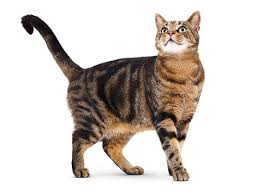
\includegraphics[width=100pt]{myimage.jpg} % width=\linewidth to get image to fill whole width

% Tout petit et centré $\rightarrow$

% \begin{center}
% %	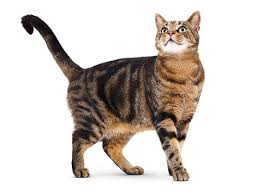
\includegraphics[width=20pt]{myimage.jpg} % width=\linewidth to get image to fill whole width
% \end{center}

% \section{Maths}

% Pour faire une équation simple, utilisez l'environnement maths. Vous pouvez faire des maths inline
% comme suit: $a = \sum_{i=0}^{N} x_i + c$ ou comme suit:

% \[ a = \sum_{i=0}^{N} x_i + c + \dfrac{1}{2} + \text{some more stuff\dots}\]


% Pour faire des équations alignées:


% \section{Et plein d'autres choses!}

% Quelques templates: \url{https://www.latextemplates.com} \\
% Documentation: \url{https://www.latex-project.org}

\begin{titlepage}
	\begin{minipage}[t]{0.3\textwidth}
		\begin{flushleft}
		\hspace{0.1cm}ET4-Info Option TAL\\
		\end{flushleft}
	\end{minipage}\hfill
	\begin{minipage}[t]{0.6\textwidth}
		\begin{flushright}
			\textsc{Mickael Francisco SERENO} \\
			\textsc{Mathieu LOUVET} \\
			\textsc{Stacy GROMAT} \\
			Promo 2018
		\end{flushright}
	\end{minipage} ~\\[1cm]

	\begin{minipage}[t]{0.5\textwidth}
		\begin{flushleft}
		\end{flushleft}
	\end{minipage}\hfill
	\begin{minipage}[t]{0.4\textwidth}
		\begin{flushright}
		\end{flushright}
	\end{minipage}\hfill
	~\\[1cm]
	\begin{center}
	 \end{center}
	 \begin{center}
	 \HRule \\[0.4cm]
		{ \huge \bfseries Rapport projet TAL \\[0.4cm] }
		\HRule \\[1cm]
	 \end{center}
		\begin{center}
		
	 \end{center}
	\vfill
	\begin{center}
		06 Mai 2017
	\end{center}
\end{titlepage}
	Introduction

  Le sujet qui a été choisi est celui du chatbot (ou assistant personnel). 
Explications sur le chat bot


L'ensemble des membres du groupe était relativement motivé par ce sujet, du chatbot. Le thème restait toutefois à choisir : pour ne pas avoir un simple robot générique

%Un chatbot/assistant personnel est un agent programm´e pour entretenir un dialogue avec un utilisateur. ` A l’origine, les chatbots ´etaient destin´es `a une tˆache sp´ecifique (p. ex. r´eservation de billets de train, assistance pour les achats dans un magasin, psychologue, etc.), mais de nos jours, il existe aussi des agents destin´es `a la conversation en g´en´eral, une tˆache bien plus difficile.
%Enjeux — Le but d’un chatbot est de cr´eer une situation de dialogue entre un utilisateur et l’agent. Son langage doit donc essayer de refl´eter le mieux possible les ´enonc´es attendus par un humain. — Veillez `a ce que les ´enonc´es que vous produisez soient grammaticalement bien form´es. Ceci peut ˆetre parfois difficile, mais fera une grande diff´erence pour la qualit´e de votre chatbot! — Des r´eponses plus pr´ecises (qui prennent en compte les ´enonc´es de l’utilisateur par exemple) augmenteront la cr´edibilit´e de votre chatbot. Un syst`eme simple qui r´ep`ere quelques mots cl´es peut ˆetre assez efficace.
%` A faire — Vous choisirez un domaine de comp´etence pour votre chatbot. Quel est est son but? Vous pouvez par exemple cr´eer un chatbot pour interroger un site de r´eservation de billets de train, pour donner des directions, ou pour entretenir une conversation. Si vous choisissez de d´evelopper un agent conversationnel g´en´eral, vous devrez probablement mettre en avant un ou deux aspects de la conversation que votre chatbot maˆıtrise particuli`erement bien. — Vous pouvez utiliser la m´ethode que vous souhaitez pour construire votre chatbot : heuristiques, motifs, mots cl´es, grammaires (CFGs avec NLTK), r´eponses g´en´eriques, etc. — les´enonc´esproduitsparvotrechatbotdevrontˆetregrammaticalementbienform´es.Faitesattention `a l’accord, aux temps des verbes, etc. — Un dialogue est form´e d’un locuteur (celui qui parle `a un instant donn´e) mais aussi d’un interlocuteur (celui qui ´ecoute). Pour cr´eer un dialogue plus r´ealiste, pensez `a inclure des ´enonc´es qui montrent que l’agent prend en compte ce que dit l’utilisateur. Les  backchannels  sont des signaux verbaux ou non verbaux qui sont les r´eponses de l’interlocuteur (hochements de tˆetes pour les agents qui ont en ont une, des marqueurs de compr´ehension tels que  uh huh ,  oui , des reprises de l’´enonc´e pr´ec´edent en cas de manque de compr´ehension etc.) — Mettez en avant ce que votre agent arrive `a faire, mais incluez dans votre rapport une section qui discute des limitations de votre chatbot : y a-t-il des choses qu’il ne peut pas g´erer? Quelle sorte de solutions proposeriez-vous pour l’avenir?

\section{Répartition des tâches}
	Au tout début du projet, nous avons réfléchis à trois pour voir comment le Chatbot serait modélisé et comment il fonctionnerait. Nous pouvons dire que le rapport est le fruit de nos trois réflexions.

	Ensuite nous avons eu globalement trois tâches:
	\begin{itemize}
		\item Récupérer les corpus ;
		\item Convertir les corpus ;
		\item Coder le ChatBot en partant des corpus convertis ;
	\end{itemize}

	Ainsi, Mathieu a récupéré les corpus via un script python, Mickael les a converti et Stacy a codé le fichier projet.py pour avoir un ChatBot.
	Quand le ChatBot a été codé, il fallait attendre que tous les corpus soient correctement traités. Cela demandait du temps car nous ne connaissions pas encore NLTK.

	Une fois les corpus convertis, nous avons pu tester le programme et nous l'avons débogué à trois, l'avons "amélioré" petit à petit (quelques petits bugs subsistaient). Il est difficile à ce stade de dire qui a fait quoi.

\section{Difficultés}


	le corpus : trouvé un corpus qui permette de mieux répondre


\clearpage
\section{Stratégie}

La stratégie envisagée est assez simple. Elle consiste à récupérer de très nombreux corpus de textes, et d'identifier dans ces écrits les couples de questions-réponses. Ensuite, une question est attendue de la part de l'utilisateur. Cette question est analysée, puis à partir d'un dictionnaire, la réponse la plus adaptée est déterminée et affichée. Pour assurer la qualité de ce chatbot, plusieurs conditions sont à assurer : 
\newline
\begin{itemize}
  \item la capacité du programme à correctement comprendre la question de l'utilisateur. Dans ce but, les phrases entrées sont divisées en ensembles linguistiques, eux-mêmes étiquetés puis pondérés. Cette pondération (cf. figure \ref{ponderationTab}) est particulièrement importante, puisque c'est elle qui permet de sélectionner la réponse la plus appropriée parmi celles possibles ;
  \item un nombre conséquent de couples de questions-réponses doit être disponible. En effet, pour répondre selon le token indiquant la question, il faut grouper l'intégralité des couples de question-réponse selon le ce token. En pratique, pour une question précise, cela divise la taille du corpus de texte utilisé par un facteur six (voire plus) ;
  \item un accès rapide aux données. Il faut qu'une réponse ne mette pas trop de temps pour revenir vers l'utilisateur. Cela implique une gestion des données performante, dont le parcours est relaitvement limité dans le temps : c'est pourquoi un dictionnaire Python (concrètement, une table de hashage) a été utilisée. Les clés de cette table de hashage sont les mots interrogatifs (reconnus par \textit{NLTK}), cela permet de diviser correctement les données.
\end{itemize}

\ 
\newline
\begin{figure}[h]
\begin{center}
\begin{tabular}{lll}
Type de token & Poids & Exemples \\
\hline
Questions & 2 & "When", "What", "Who", "Where", "Why", "How"\\
Verbes & 1.2 & "Borrow", "Expand" \\
Noms & 0.7 & "John", "Doe" \\
Pronoms & 0.7 & "You", "Themself" \\
Adjectifs & 0.25 & "Awesome", "Magnificent" \\ 
Adpositions & 0.25 & "From", "With" \\
Adverbes & 0.25 & "Certainly", "Even" \\
Autres & 0 & "?", "msitake", "666", \dots \\
\end{tabular}
\caption{Tableau de pondération des éléments syntaxiques}
\label{ponderationTab}
\end{center}
\end{figure}

\subsection{Les différentes pondérations}

Il paraissait évident d'attribuer différent poids aux différents, mais pourquoi de tels choix de pondération ? Voici une explication selon les types de tokens identifiés par \textit{NLTK} : \newline

\begin{description}
  \item[Questions :] Détermine la nature de la réponse et sa tournure principale. C'est pourquoi la pondération de ce type d'éléments a été majorée ;
  \item[Verbes :] Fixe le type d'action et permet généralement d'identifier l'action ou l'évènement concerné(e) par la question. Il permet de réduire correctement les réponses possibles : c'est pourquoi il s'agit de la seconde plus grande pondération ;
  \item[Noms :] Un nom fait souvent référence à un contexte précis, ou tout simplement à un interlocuteur, parfois direct. C'est pourquoi il est important. Toufefois, si un nom n'est pas trouvé dans la base de données, il devient immédiatement sans importance. Cela devrait être fréquent, puisqu'il existe une infinité de noms propres. De plus, certains noms sont beaucoup plus fréquents que d'autres. Si une importance trop grande était accordée aux noms, alors une réponse en rapport avec ce nom, mais totalement hors-sujet pourrait être fournie ;
  \item[Pronoms :] Les pronoms sont bien plus permissifs que les noms en termes de réponses. C'est pourquoi leur poids n'est pas non plus extrêmement important. De plus, ils sont utilisés dans beaucoup de contextes, sans forcément avoir une importance majeure. Par exemple, lors d'une tournure rhétorique anglaise "..., don't you?", l'information principale de la phrase est contenue dans la partie initiale de la phrase. Bien qu'une réponse courte du type "I do" soit valide, d'un point de vue conversationnel, il est plus intéressant de s'intéresser aux autres éléments de la phrase ; 
  \item[Adjectifs :] La majorité des adjectifs peuvent être remplacés par d'autres adjectifs sans forcément changer le sens de la phrase. C'est pourquoi ils ont un poids relativement faible. Néanmoins, la présence d'un champ lexical pour connaître les adjectifs permettrait d'élargir le champ de recherche des réponses vlaides en évitant en même temps les adjectifs qui changent effectivement le sens de la phrase ;
  \item[Adverbes :] Les adverbes correspondent à un cas relativement similaire à celui des adjectifs, explicant leur poids faible ;
  \item[Adpositions :] Les adpositions correspondent généralement à un complément d'information à l'action. Action qui reste l'un des éléments principaux de la phrase. Les adpositions ont donc une pondération faible ;
  \item[Autres :] Les autres types de tokens comprennent les conjonctions, les déterminants, les nombres cardinaux, les particules, les mots issus d'une autre langue et enfin les fautes de frappes sont actuellement très peu importants à la réponse. En guise d'illustration, changer un nombre de valeur n'affecte que très peu le sens de la phrase (bien que les conséquences puissent être totalement différente selon le contexte). Toutefois, la pondération n'est pas nulle, juste très faible, car certains de ces mots pourraient revenir plusieurs fois dans une seule et même phrase, cela la mettrait en avant face à d'autres phrases similaires comportant moins de fois ces mots.

  Les signes de ponctuation sont volontaires omis (pondération quasi-nulle) puisque l'entrée doit être similaire à une question pour que le programme trouve une réponse adaptée.
\end{description}

\subsection{Une capture d'écran puis suite?} 
\newpage
\section{Améliorations possibles}
\subsection{Maintenir une analyse constante}
Voici le scénario envisagé. L'utilisateur pose une question, le programme lui fournit une réponse. Une autre question est entrée, une nouvelle réplique est affichée. Et ainsi de suite. Pourquoi ne pas exploiter ce défilement d'informations potentiellement nouvelles ?
\subsubsection{Enregistrer les entrées de l'utilisateur}
	Supposons que le programme échoue à analyser ou à répondre à l'utilisateur. Il pourrait demander à l'utilisateur de fournir une réponse convenable à sa question, et ainsi enregistrer un nouveau couple de question réponse.

	Ou de manière bien plus transparente, il pourrait analyser la réaction de l'utilisateur suite à sa propre réponse. Il faudrait bien sûr une base de réponses désignant l'incompréhension, composée de phrases telles que "ce que tu dis n'a aucun sens" ou encore "tu racontes n'importe quoi". Si la machine reconnait une de ces phrases, elle stockerait une nouvelle association de question-réponse dans une table "à ne pas faire". Cette association doit avoir une valeur de fréquence, pour mesurer l'importance de cette réponse jugée inappropriée. En effet, certaines réponses de ce type pourraient relever du sarcasme (les smileys textuels ne sont absolument pas analysés).
\subsubsection{Suivre un fil conducteur}
	L'idée est ici de mettre en place un historique et de l'analyser pour maintenir un lien concret entre une suite de question. Il pourrait être tout à fait pertinent que le programme se concentre sur certains thèmes ou champs lexicaux de la base de données.
	Par exemple, si la conversation est particulièrement orientée "sciences appliquées", il serait intéressant de favoriser les répliques provenant d'Interstellar et autres scripts issus de films ayant ce thème.

	Concrètement, cela nécessiterait un travail de catégorisation des scripts, qui devrait se révéler relativement aisé, puisque les films sont généralement classés par genre. Mais comme les thèmes sont multiples et variés, d'autres méthodes sont certainement préférables.

\subsection{Utilisation de champs lexicaux}%Créer de nouvelles phrases, ou élargir de le champ de recherche.
	Une de ces méthodes serait l'analyse de la question non pas seulement par sa probabilité de réponse selon un corpus de texte qui va finir par devenir volumineux, mais également par le champ lexical des mots de la phrase. En effet, connaître le champ lexical des noms communs, des adjectifs ou des verbes permettrait d'élargir le champ de recherche de réponse à cette question.

	Cependant, cet élargissement du champ de recherche risquerait d'alourdir considérablement le temps de réponse, puisqu'il faudrait comparer toutes les phrases possibles pour obtenir la (ou l'une des) meilleure(s). Si ce temps d'attente reste tolérable, alors cette implémentation devrait être valide. A contrario, si la machine ne rétorque pas suffisamment vite, il faut envisager d'autres solutions.

	L'une d'entre elles serait la génération de phrases. En pratique, le champ lexical n'est pas très long à récupérer si un système performant existe déjà. Le British Lexicon Project devrait a priori pouvoir aider sur ce point. Pour générer une phrase correcte, il suffirait de voir la structure de phrase la plus fréquente (à l'aide des tags \textit{NLTK}), et de piocher dans le champ lexical des mots correspondant au type de token pour constituer une nouvelle phrase. Il s'agit bien sûr d'une méthode relativement basique ici, et d'autres plus élaborées existent certainement.

\subsection{Correction orthographique}
Une ultime amélioration apparente est celle de la correction orthographique des entrées de l'utilisateur. La manière transparente de faire serait d'accepter l'entrée de l'utilisateur, telle qu'elle est et d'y appliquer le correcteur orthographique dans l'espoir qu'il ne fasse pas d'erreur. Cette manière fonctionne particulièrement bien avec un unique (profil d') utilisateur, puisque via un processus d'apprentissage automatique, elle se familiarise avec le vocabulaire de l'individu (un des meilleurs exemples de ceci est le correcteur orthographique des smartphones).

De même, une solution valide serait de suggérer à l'utilisateur des corrections potentielles (via une interface graphique), qu'il sélectionnerait (l'illustration est ici le correcteur grammatical de Microsoft Office Word ou LibreOffice Writer).

Comment seraient suggérées ces corrections ? À l'aide d'un calcul de distance de Levenshtein, qui permet de calculer la similitude entre deux mots, en détectant les permutations, ajouts et suppressions de lettres pour arriver d'un mot à un autre. L'algorithme est relativement simple, mais s'il est appliqué à tout un dictionnaire, il risquerait d'être particulièrement gourmand en ressources. Limiter la corrections à trois ou quatre mots très proche semble raisonnable.

\section{Exemple d'exécution}

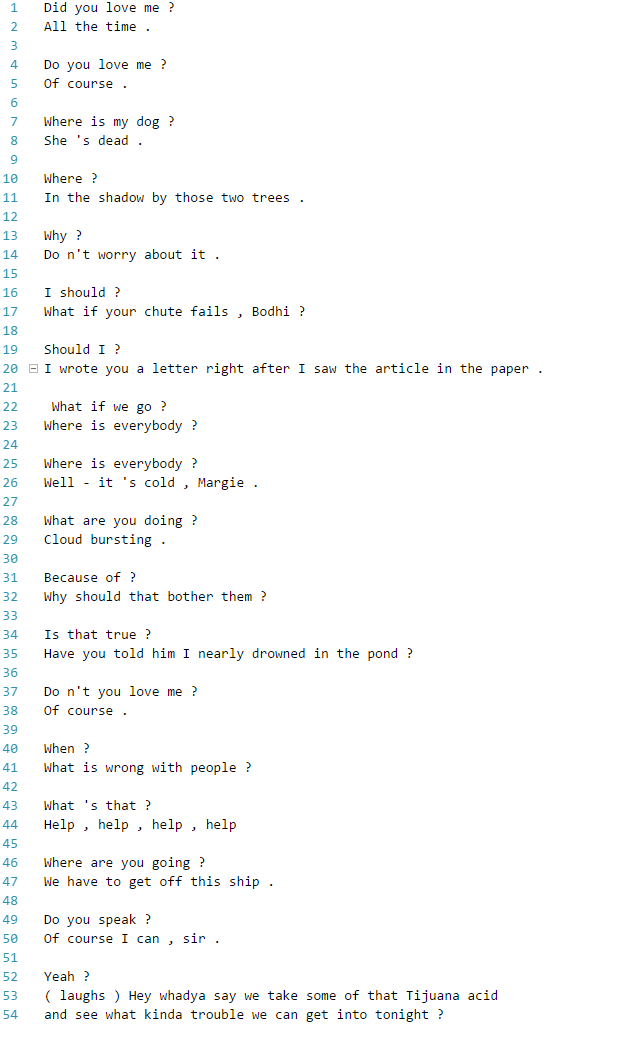
\includegraphics[scale=0.85]{executionCapture.PNG}
\end{document}
